%\item Une unité de cavalerie peut, à l'issue de son déplacement, initier une attaque contre une unité ennemie se trouvant sur une des 8 cases adjacentes à cette unité de cavalerie afin d'utiliser sa charge. La charge de cavalerie donne un coefficient offensif de 7 à cette unité de cavalerie et permet de faire participer à l'offensive les autres unités de cavalerie alliées se trouvant dans le même alignement de cases sans discontinuité de cases entre elles. Ainsi les unités de cavalerie participant à la charge voient leurs coefficients offensifs montés à 7.



% sémantique/commandes de l'utilisateur
% -Load
% -Save
% -Move
% -Attack
% (Spécifier des options de début de partie ?)
% (Placer les unités au début de la partie ?)
% 
%Si les besoins primaires consistent seulement dans l'implémentation d'un moteur de règle fonctionnel, il faut pouvoir lui donner un plateau, avec lequel il pourra communiquer, et donc prévoir aussi ça...


% revoir priorités again
%Le projet se divise donc en deux parties, après avoir une version jouable du \textit{Jeu de la Guerre} entre deux utilisateurs sur une même console, il est désormais question d'ajouter des aides aux joueurs et des interactions avec l'interface graphique.

%Il s'agit d'étendre l'implémentation actuelle pour permettre de pouvoir jouer une partie complète sur le programme en utilisant des aides à la compréhension d'une situation.

%Ces aides permettront à l'utilisateur d'appréhender plus facilement et rapidement la situation de la partie, à savoir par exemple, mais peut-être pas limité à, le potentiel offensif et défensif de chaque case du plateau, la portée des lignes de communications, la portée d'attaque des unités. Ces aides ne devront pas être exclusivement visuelle et pourront être utilisées par un potentiel joueur artificiel plus tard.

%L'utilisateur sera en mesure de jouer toute une partie via l'interface graphique à l'aide de sa souris. Il pourra ainsi interagir avec ses unités mais aussi sélectionner les aides à afficher/enlever sur le plateau à l'aide d'un menu déroulant par exemple.
%\newline

%Ainsi les besoins pour cette partie sont les suivants :

%Le joueur artificiel devra reconnaître l'ensemble des coups possibles à son tour, et pouvoir les jouer en pouvant utiliser des heuristiques qui seront détaillées dans les besoins tertiaires. Dans ce premier temps, on pourra par exemple, limiter ces heuristiques et plutôt jouer les coups de façon aléatoire.

%\subsection*{PdP 2015\cite{pdp2015}}
%Ce projet fournit une batterie de tests non-exhaustive de l'implémentation des règles du jeu de la guerre du groupe. Le projet a subit des problèmes au sein du groupe et est resté inachevé.


% intro
% En plus du livre écrit par Debord, il existe déjà des documents liés à notre projet :

% \section{Kriegspiel}

% Le jeu \href{http://r-s-g.org/kriegspiel/index.php}{Kriegspiel} également basé sur le jeu de Guy Debord.


%L'objectif premier à réaliser, et le grand pilier du projet, consiste à implémenter de façon informatique les règles du Jeu de la guerre en respectant autant que possible les idées de Guy Debord, dans une sorte de moteur de règles qui permet d'affirmer si un coup donné par un joueur à un moment donné d'une partie est valide ou non. Cette implémentation devra pouvoir rendre possible l'extension du moteur pour les besoins secondaires et tertiaires ainsi que posséder une interface permettant à un utilisateur d'interagir avec le programme.
%\newline

%Les besoins et contraintes de programmation apportés par cette première partie sont les suivants :


%\item À son tour avant le début de la partie, l'utilisateur devra positionner ses unités sur le plateau sans que la position de l'armée adverse lui soit montrée.

%\item Dans la phase de positionnement des unités, l'utilisateur pourra déplacer ses unités déjà placées sur le plateau sans limitation dans sa zone à l'aide de la commande permettant le déplacement d'une unité.

%\item Les unités sont désignées de la façon suivante : (voir figure \ref{fig:commands})
%	\begin{itemize}
%	\item Le régiment d'infanterie : \texttt{I}
 %   \item Le régiment de cavalerie : \texttt{C}
  %  \item Le régiment d'artillerie à pied : \texttt{A}
   % \item Le régiment d'artillerie à cheval : \texttt{Ac}
    %\item L'unité de communication à pied : \texttt{R}
%    \item L'unité de communication à cheval : \texttt{Rc}
 %   \item Une montagne : \texttt{M}
  %  \item Un col : \texttt{Co}
   % \item Une forteresse : \texttt{F}
    %\item Un arsenal : \texttt{Ar}
	%\end{itemize}
% ^ commenting de qualité

%<Joueur Actuel> <Nombre de coups restant>
%<ID d'un décor>;<X>;<Y>;<Est cassé>;<Joueur>
%<ID de l'unité>;<X>;<Y>;<Doit bouger>;<A bougé>;<A attaqué>;<Joueur>


%\item Toujours durant cette phase, l'utilisateur pourra repositionner une unité sur le plateau sur une autre case, un échange de position se fera si la case ciblée est occupée par une unité alliée.

%%% Priorité 1 - Interface minimale (console) pour joueurs
% Afficher et expliquer les règles vérifiées et leur validité
% + étape de validation par le joueur d'un coup affirmé valide ? (test/simulation de coup)

  %\item Permettre à deux utilisateurs de jouer dans une même console à tour de rôle.
  
  %\item À son tour, l'utilisateur devra proposer une action en utilisant une syntaxe à définir.
  
  %\item Le programme générera et affichera un aperçu de la situation représentant l'état du plateau après chaque coup valide joué (nature de l'aperçu à définir ultérieurement).
  
  %\item Toujours avec cette syntaxe, un joueur devra pouvoir annuler les derniers coups qu'il a joué, jusqu'à revenir au début de son tour s'il le souhaite. (Ce mécanisme pourra être implémenté à l'aide d'une pile des instances du plateau pendant ce tour). % voir avec test/simulation
  
  %\item Un joueur pourra sauvegarder l'état du plateau dans un fichier en respectant un ordre logique des informations stockées, lisible par l'utilisateur.
  %\item Un joueur pourra générer une instance du jeu à partir d'un fichier suivant un format défini.
  %\item Une première IA sera implémentée. Elle sera en lien avec le moteur de règle et pourra récupérer la liste des coups valides, pourra proposer des actions au jeu et devra pouvoir être étendable. %(étendue facilement)

%Cette dernière partie du projet se focalise sur le joueur artificiel exclusivement, afin de pouvoir le faire jouer de façon efficace en utilisant des notions tactiques et stratégiques \cite{AI2009}. Il faudra probablement faire interpréter une situation donnée au joueur artificiel pour que celui-ci prenne une décision pertinente dans un temps réduis. On pourra penser par exemple à représenter les unités des deux joueurs par des "ensembles d'unités à un certain potentiel".
%Dans cette partie, il s'agira de se focaliser sur un analyseur, utilisant des données telle que la cartographie des coefficients d'attaque, dont le but sera de pouvoir calculer un ou plusieurs coups à partir d'une situation donnée, en utilisant des notions stratégiques \cite{AI2009} pour lui faire mettre en place une tactique.
%\newline 

%M. Narbel nous a notamment indiqué les deux besoins concernant une stratégie potentielle pour un joueur artificiel : %TBC
%\newline


%D'autres stratégies pourront être mises en place si le temps le permet, à savoir mesurer l'agressivité et le positionnement des troupes de l'adversaire (réduction à une dimension pour chacun des axes), et de détecter les tactiques "commando", comme remarqué avec le détachement de l'unité de Cavalerie dans la partie présentée par Debord dans son livre (voir \cite{jdg}, pages 11-127).

%Ces stratégies et tactiques pourront être utilisées comme représentation graphique pour conseiller le joueur (aperçus types "schémas militaires"), ainsi que comme une série d'indications pour un potentiel joueur artificiel.
   
% Une première IA | <- QUI A OSÉ ??| sera implémentée. Elle sera en lien avec le moteur de règle et pourra récupérer la liste des coups valides, pourra proposer des actions au jeu et devra pouvoir être étendable. %(étendue facilement)

%\begin{figure}[h]
%\caption{Diagramme de séquence pour un coup valide proposé}
%\centering
%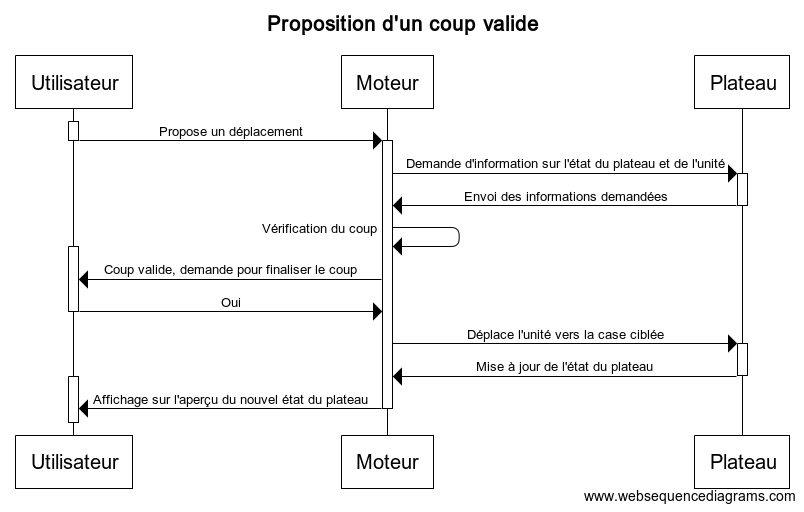
\includegraphics[width=0.8\textwidth]{sequence}
%\label{fig:scenario1}
%\end{figure}


% \section{Besoins accessoires}
% % wtf
% Pour améliorer le projet si les besoins les plus importants ont été accomplis, plusieurs idées peuvent être mises en oeuvre :

% \begin{itemize}
% \item Une représentation graphique 2D du jeu, avec diverses aides visuelles telles que l'affichage des lignes de communication et la puissance des unités.
% \end{itemize}


% Classer les règles du jeu et l'ordre dans lequel on doit les implémenter

%\item Le module de moteur de règles sera composé d'un ensemble de règles et s'occupe de modifier l'état du plateau sur le déroulement d'une partie.

%\item Le module d'interface utilisateur offrira un environnement utilisable par l'utilisateur pour interagir avec le jeu. Les interactions avec le moteur de jeu seront définies par une interface (représentée par \texttt{Player}) qui sera aussi utilisée aussi bien que par un joueur humain que par un potentiel joueur artificiel. Cet environnement sera dans un premier temps une interface console affichant l'état du plateau dans une fenêtre à part, puis une interface graphique après la première release. %%TODO ?

% \item Le module d'IA sera composé de "comportements" et interagira avec le moteur de règles pour avoir les informations sur l'état de la partie pour décider du coup à jouer. Les fonctionnalités pour obtenir ces informations pourront être utilisées aussi par le module d'interface utilisateur afin d'afficher les aides visuelles comme les portées d'attaque, les valeurs de défense des unités, etc...

%\item Le module d'Analyse permettra d'obtenir des informations et données stratégiques et tactiques sur une situation donnée et sur les tours précédents. L'idéal serait de pouvoir proposer des stratégies ou tactiques à partir de ces informations, pouvant être ultimement employé par un joueur artificiel.

%\item Le module de plateau est une sorte de conteneur qui s'occupe de gérer l'état du plateau, de l'exporter et de l'importer. Il ne doit pas être accessible par les autres classes Analyse et Interface Utilisateur pour éviter la perte de cohérence sur le déroulement de la partie. Restreindre l'accès au Plateau uniquement au moteur de jeu force les autres modules à passer par la vérification des règles avant d'agir sur le terrain.


%\item Le développement des différentes étapes non triviales devra être conduit par groupes de 2 (voir le diagramme \ref{fig:gantt}) développeurs pour garder une cohérence, pas plus pour éviter les ralentissements sur une seule partie du code, mais pas moins non plus pour avoir un code maintenable et compris par plusieurs développeurs.

%\item Les deux dernières semaines du projet seront réservées à la rédaction du mémoire ainsi que pour compenser le retard éventuel généré lors du développement.



